%%% Template originaly created by Karol Kozioł (mail@karol-koziol.net) and modified for ShareLaTeX use

\documentclass[a4paper,11pt]{article}

\usepackage[T1]{fontenc}
\usepackage[utf8]{inputenc}
\usepackage{graphicx}
\usepackage{xcolor}

\usepackage{sansmath}
\renewcommand\familydefault{\sfdefault}
\usepackage{tgheros}

\usepackage{amsmath,amssymb,amsthm,textcomp}
\usepackage{enumerate}
\usepackage{multicol}
\usepackage{tikz}
\usetikzlibrary{shapes, positioning}

\usepackage{geometry}
\geometry{total={210mm,297mm},
left=25mm,right=25mm,%
bindingoffset=0mm, top=20mm,bottom=20mm}


\linespread{1.3}

\newcommand{\linia}{\rule{\linewidth}{0.5pt}}

% custom theorems if needed
\newtheoremstyle{mytheor}
    {1ex}{1ex}{\normalfont}{0pt}{\scshape}{.}{1ex}
    {{\thmname{#1 }}{\thmnumber{#2}}{\thmnote{ (#3)}}}

\theoremstyle{mytheor}
\newtheorem{defi}{Definition}

% my own titles
\makeatletter
\renewcommand{\maketitle}{
\begin{center}
\vspace{2ex}
{\huge \textsc{\@title}}
\vspace{1ex}
\\
\linia\\
\@author \hfill \@date
\vspace{4ex}
\end{center}
}
\makeatother
%%%

% custom footers and headers
\usepackage{fancyhdr}
\pagestyle{fancy}
\lhead{}
\chead{}
\rhead{}
\lfoot{Automatic~Verification Assignment \#1}
\cfoot{}
\rfoot{Page \thepage}
\renewcommand{\headrulewidth}{0pt}
\renewcommand{\footrulewidth}{0pt}
%

% all section titles centered and bolded
\usepackage{sectsty}
\allsectionsfont{\bfseries\large}
%
% add section label
\renewcommand\thesection{Problem~\arabic{section}:}
%

%%%----------%%%----------%%%----------%%%----------%%%

\begin{document}

\title{Homework Assignment~\#1}

\author{R02943142 Hsieh, Chiao}

%\date{01/01/2014}

\maketitle

\section{CTL Model Checking}
Consider model checking the CTL property 
$\textbf{AG}((at\ l_0) \to \textbf{AF}(at\ CR_0))$
(using the CTL model checking procedures in Chapter 4.1 of [CGP]) against the
following Kripke structure which represents a two-process mutual exclusion
algorithm using an atomic read/write variable.
\medskip \\
Answer.
\smallskip \\
First, we normalize the property.
\smallskip \\
$
\textbf{AG}(l_0 \to \textbf{AF}(CR_0)) \\
= \neg \textbf{EF} \neg (\neg l_0 \lor \neg \textbf{EG}(\neg CR_0)) \\
= \neg \textbf{E} [ true\ \textbf{U}\ \neg (\neg l_0 \lor \neg \textbf{EG}(\neg CR_0)) ]
$
\smallskip \\
Then, following sub-formulae are going to be labeled one by one on each state 
according to the model checking algorithm.\\
$
\{
\textbf{EG}(\neg CR_0), 
(\neg l_0 \lor \neg \textbf{EG}(\neg CR_0)),
\textbf{E} [ true\ \textbf{U}\ \neg (\neg l_0 \lor \neg \textbf{EG}(\neg CR_0)) ]
\}
$
\smallskip \\
To simplify the labels on graph, let \\
$
p0 = \textbf{EG}(\neg CR_0), \\
p1 = (\neg l_0 \lor \neg p0), \\
p2 = \textbf{E} [ true\ \textbf{U}\ \neg p1) \\
\Rightarrow \textbf{AG}(l_0 \to \textbf{AF}(CR_0)) = \neg p2
$

To label $p0$, the new machine $M'$ is derived by simply deleting the two 
states labeled with $CR_0$ and their incoming and outgoing edges. The
corresponding strongly connected components~(SCC) are then computed~(See graph
below). Each of them is a single node with a self-loop. Apparently, all states 
in $M'$ can reach a SCC, so all states in $M'$ are labeled with $p0$.

\begin{center}
\tikzstyle{every node}=[ellipse, inner sep=1pt, draw, font=\tiny, align=center, minimum width=40pt]
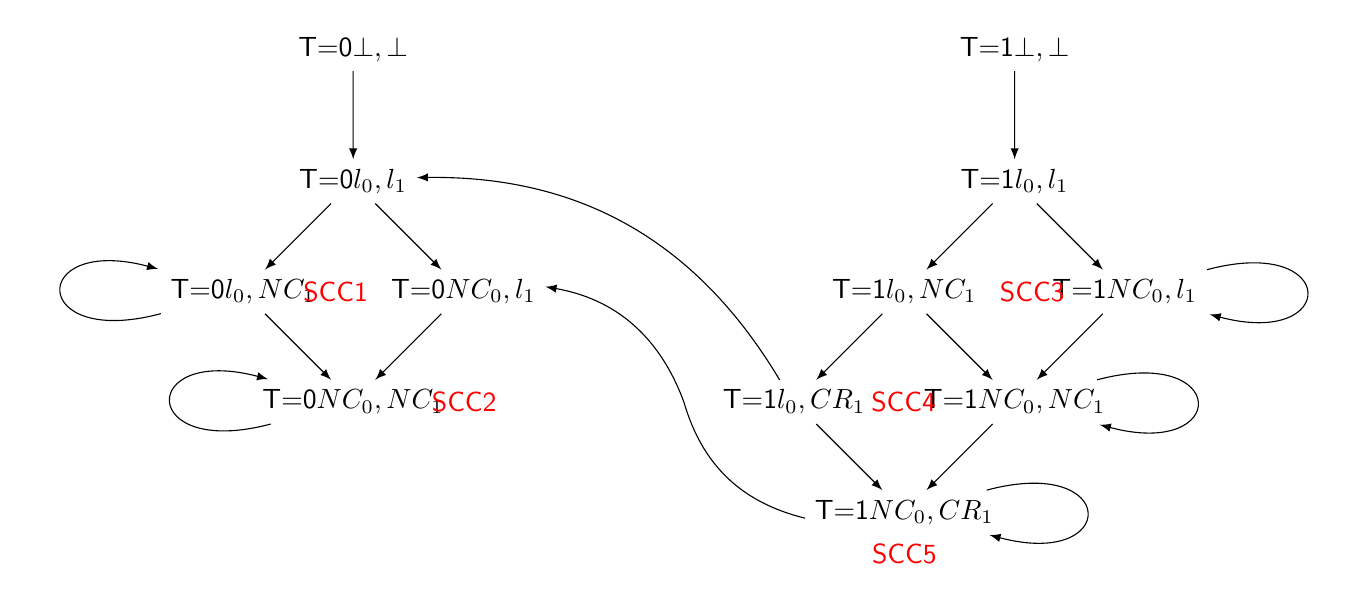
\begin{tikzpicture}[->,>=latex, auto, scale=1.4]
  \node (P0_0) at (1, 4.2) {T=0 \\ $\bot, \bot$};
  \node (P0_1) at (1, 3) {T=0 \\ $l_0, l_1$};
  \node (P0_2) at (0, 2) {T=0 \\ $l_0, NC_1$};
    \node [draw=none, text=red, right = -0.4 of P0_2] {SCC1};
  \node (P0_3) at (2, 2) {T=0 \\ $NC_0, l_1$};
  \node (P0_4) at (1, 1) {T=0 \\ $NC_0, NC_1$};
    \node [draw=none, text=red, right = -0.4 of P0_4] {SCC2};


  \node (P1_0) at (7, 4.2) {T=1 \\ $\bot, \bot$};
  \node (P1_1) at (7, 3) {T=1 \\ $l_0, l_1$};
  \node (P1_2) at (6, 2) {T=1 \\ $l_0, NC_1$};
  \node (P1_3) at (8, 2) {T=1 \\ $NC_0, l_1$};
    \node [draw=none, text=red, left = -0.4 of P1_3] {SCC3};
  \node (P1_4) at (7, 1) {T=1 \\ $NC_0, NC_1$};
    \node [draw=none, text=red, left = -0.4 of P1_4] {SCC4};
  \node (P1_5) at (5, 1) {T=1 \\ $l_0, CR_1$};
  \node (P1_6) at (6, 0) {T=1 \\ $NC_0, CR_1$};\
    \node [draw=none, text=red, below = 0 of P1_6] {SCC5};

  \path
    (P0_0) edge (P0_1)
    (P0_1) edge (P0_2)
           edge (P0_3)
    (P0_2) edge [loop left] (P0_2)
           edge (P0_4)
    (P0_3) edge (P0_4)
    (P0_4) edge [loop left] (P0_4)

    (P1_0) edge (P1_1)
    (P1_1) edge (P1_2)
           edge (P1_3)
    (P1_2) edge (P1_4)
           edge (P1_5)
    (P1_3) edge [loop right] (P1_3)
           edge (P1_4)
    (P1_4) edge [loop right] (P1_4)
           edge (P1_6)
    (P1_5) edge (P1_6)
           edge [bend right] (P0_1)
    (P1_6) edge [loop right] (P1_6)
    ;

  \draw (P1_6) to [bend left] (4, 1) to [bend right] (P0_3);
\end{tikzpicture}
\end{center}

\begin{center}
\tikzstyle{every node}=[ellipse, inner sep=1pt, draw, font=\tiny, align=center, minimum width=40pt]
\tikzstyle{ap}=[draw=none, text=blue]
\begin{tikzpicture}[->,>=latex, auto, scale=1.4]
  \node (P0_0) at (1, 4.2) {T=0 \\ $\bot, \bot$};
    \node[ap, above = 0 of P0_0] {$\{p0, p1, p2\}$};
  \node (P0_1) at (1, 3) {T=0 \\ $l_0, l_1$};
    \node[ap, above left = 0 of P0_1] {$\{p0, \neg p1, p2\}$};
  \node (P0_2) at (0, 2) {T=0 \\ $l_0, NC_1$};
    \node[ap, above = 0 of P0_2] {$\{p0, \neg p1, p2\}$};
  \node (P0_3) at (2, 2) {T=0 \\ $NC_0, l_1$};
    \node[ap, above = 0 of P0_3] {$\{p0, p1, p2\}$};
  \node (P0_4) at (1, 1) {T=0 \\ $NC_0, NC_1$};
    \node[ap, below = 0 of P0_4] {$\{p0, p1, p2\}$};
  \node (P0_5) at (3, 1) {T=0 \\ $CR_0, l_1$};
    \node[ap, below = 0 of P0_5] {$\{\neg p0, p1, p2\}$};
  \node (P0_6) at (2, 0) {T=0 \\ $CR_0, NC_1$};
    \node[ap, below = 0 of P0_6] {$\{\neg p0, p1, p2\}$};

  \node (P1_0) at (7, 4.2) {T=1 \\ $\bot, \bot$};
    \node[ap, above = 0 of P1_0] {$\{p0, p1, p2\}$};
  \node (P1_1) at (7, 3) {T=1 \\ $l_0, l_1$};
    \node[ap, above left = 0 of P1_1] {$\{p0, \neg p1, p2\}$};
  \node (P1_2) at (6, 2) {T=1 \\ $l_0, NC_1$};
    \node[ap, above = 0 of P1_2] {$\{p0, \neg p1, p2\}$};
  \node (P1_3) at (8, 2) {T=1 \\ $NC_0, l_1$};
    \node[ap, above = 0 of P1_3] {$\{p0, p1, p2\}$};
  \node (P1_4) at (7, 1) {T=1 \\ $NC_0, NC_1$};
    \node[ap, below = 0 of P1_4] {$\{p0, p1, p2\}$};
  \node (P1_5) at (5, 1) {T=1 \\ $l_0, CR_1$};
    \node[ap, below = 0 of P1_5] {$\{p0, p1, p2\}$};
  \node (P1_6) at (6, 0) {T=1 \\ $NC_0, CR_1$};
    \node[ap, below = 0 of P1_6] {$\{p0, p1, p2\}$};

  \path
    (P0_0) edge (P0_1)
    (P0_1) edge (P0_2)
           edge (P0_3)
    (P0_2) edge [loop left] (P0_2)
           edge (P0_4)
    (P0_3) edge (P0_4)
           edge (P0_5)
    (P0_4) edge [loop left] (P0_4)
           edge (P0_6)
    (P0_5) edge (P0_6)
           edge [bend left] (P1_1)
    (P0_6) edge [loop left] (P0_6)

    (P1_0) edge (P1_1)
    (P1_1) edge (P1_2)
           edge (P1_3)
    (P1_2) edge (P1_4)
           edge (P1_5)
    (P1_3) edge [loop right] (P1_2)
           edge (P1_4)
    (P1_4) edge [loop right] (P1_4)
           edge (P1_6)
    (P1_5) edge (P1_6)
           edge [bend right] (P0_1)
    (P1_6) edge [loop right] (P1_6)
    ;

  \draw (P0_6) to [bend right] (4, 1) to [bend left] (P1_2);
  \draw (P1_6) to [bend left] (4, 1) to [bend right] (P0_3);
  
\end{tikzpicture}
\end{center}

For $p1$, we just label those states that without either $l_0$ or $p0$, and 
then for $p2$, we backward find all states that can reach states labeled with 
$\neg p1$, i.e., states not labeled with $p1$.
The final labeled graph is shown as above. Because both initial states are
labeled with $p2$, it is clear that $\textbf{AG}(l_0 \to \textbf{AF}(CR_0))$
does not hold.

In order to prevent the starvation problem, fair computations should frequently 
visit the two states labeled with $CR_0$. Hence, the fairness constraint $F$ 
must have at least a set $P$ containing these two states. Under this constraint,
there is no fair non-trivial SCC when computing \textit{CheckEG} procedure for 
$p0$. Therefore, all states are labeled with $\neg p0$ and hence $p1$. Since all
states are labeled with $p1$, no state can eventually reach a state labeled with
$\neg p1$; thus all states are labeled with $\neg p2$, and this implies
$\textbf{AG}(l_0 \to \textbf{AF}(CR_0))$ always holds

\section{LTL Model Checking}
Consider another two-process mutual exclusion algorithm via the arbitration
of a binary sema-phore. The Kripke structure representing this system is as
follows.
\begin{center}
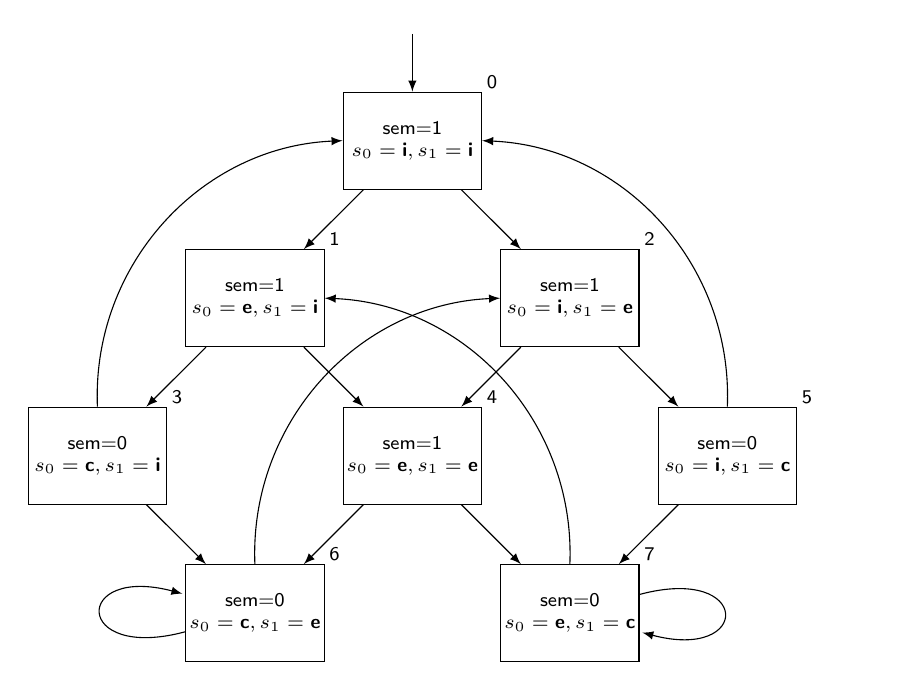
\begin{tikzpicture}[
  ->,>=latex, auto, scale=2,
  every node/.style={
    rectangle, inner sep=1pt, draw, font=\scriptsize,
    align=center, minimum width=50pt, minimum height=35pt
  },
  every label/.style={
    draw=none, label distance=-20pt
  }
]
  \node [draw=none, minimum width=0pt, minimum height=0pt] (init) at (2, 3.7)
        {};
  \node [label=above right:0] (s0) at (2, 3)
        {sem=1 \\ $s_0=\textbf{i}, s_1=\textbf{i}$};
  \node [label=above right:1] (s1) at (1, 2)
        {sem=1 \\ $s_0=\textbf{e}, s_1=\textbf{i}$};
  \node [label=above right:2] (s2) at (3, 2)
        {sem=1 \\ $s_0=\textbf{i}, s_1=\textbf{e}$};
  \node [label=above right:3] (s3) at (0, 1)
        {sem=0 \\ $s_0=\textbf{c}, s_1=\textbf{i}$};
  \node [label=above right:4] (s4) at (2, 1)
        {sem=1 \\ $s_0=\textbf{e}, s_1=\textbf{e}$};
  \node [label=above right:5] (s5) at (4, 1)
        {sem=0 \\ $s_0=\textbf{i}, s_1=\textbf{c}$};
  \node [label=above right:6] (s6) at (1, 0)
        {sem=0 \\ $s_0=\textbf{c}, s_1=\textbf{e}$};
  \node [label=above right:7] (s7) at (3, 0)
        {sem=0 \\ $s_0=\textbf{e}, s_1=\textbf{c}$};

  \path
    (init) edge (s0)
    (s0) edge (s1) edge (s2)
    (s1) edge (s3) edge (s4)
    (s2) edge (s4) edge (s5)
    (s3) edge (s6) edge [bend left =45] (s0)
    (s4) edge (s6) edge (s7)
    (s5) edge (s7) edge [bend right=45] (s0)
    (s6) edge [loop left ] (s6) edge [bend left =45] (s2)
    (s7) edge [loop right] (s7) edge [bend right=45] (s1)
    ;
\end{tikzpicture}
\end{center}

Check if the system at state 1 satisfies the LTL formula
$\textbf{A}((s_0 = \textbf{e}) \textbf{U} (s_0 = \textbf{c}))$ (using the LTL
model checking procedures in Chapter 4.2 of [CGP]). Please illustrate the model
checking steps by giving the closure of the formula, relevant parts of the
product graph (composed from the Kripke structure and the implicit tableau),
etc.
\medskip \\
Answer.

To falsify the property 
$\textbf{A}[(s_0 = \textbf{e}) \textbf{U} (s_0 = \textbf{c})]$, we try to prove $\textbf{E}\neg[(s_0 = \textbf{e}) \textbf{U} (s_0 = \textbf{c})]$.
Following the LTL model checking procedure, we first compute the closure of
$\neg [(s_0 = \textbf{e}) \textbf{U} (s_0 = \textbf{c})]$ and list these
formulae.
\smallskip \\
$
CL(\neg[(s_0 = \textbf{e}) \textbf{U} (s_0 = \textbf{c})]) = \{ \\
\neg [(s_0 = \textbf{e}) \textbf{U} (s_0 = \textbf{c})],
[(s_0 = \textbf{e}) \textbf{U} (s_0 = \textbf{c})], \\
(s_0 = \textbf{e}), \neg (s_0 = \textbf{e}),
(s_0 = \textbf{c}), \neg (s_0 = \textbf{c}), \\
\textbf{X}[(s_0 = \textbf{e}) \textbf{U} (s_0 = \textbf{c})],
\neg \textbf{X}[(s_0 = \textbf{e}) \textbf{U} (s_0 = \textbf{c})],
\textbf{X} \neg [(s_0 = \textbf{e}) \textbf{U} (s_0 = \textbf{c})],
\neg \textbf{X} \neg [(s_0 = \textbf{e}) \textbf{U} (s_0 = \textbf{c})] \\
\}
$

Next, we compute the set of atoms for constructing the behavior graph. Observe 
that the property only considers the value of $s_0$; hence, those states labeled
with same value of $s_0$ should derive very similar maximal consistent set of 
formulae, $K$, and the only difference comes from the atomic proposition on each
state. Below is the computed $K$ for different value of $s_0$. For each 
state $j$, we can derive $K_j$ by disjunction of $L(j)$ and $K$ with 
the same value of $s_0$ in $L(j)$. E.g. we can derive $K_0$ for state 0 by $K_0 = L(0) \cup K_{s_0=\textbf{i}}$.

\medskip
\noindent State 0, 2, 5: $s_0 = \textbf{i}$\\
$
K_{s_0=\textbf{i}}' = \{
\neg(s_0 = \textbf{e}), \neg(s_0 = \textbf{c}),
\neg[(s_0 = \textbf{e}) \textbf{U} (s_0 = \textbf{c})],
\neg \textbf{X} [(s_0 = \textbf{e}) \textbf{U} (s_0 = \textbf{c})],
\textbf{X} \neg [(s_0 = \textbf{e}) \textbf{U} (s_0 = \textbf{c})]
\}
$
\\
$
K_{s_0=\textbf{i}}'' = \{
\neg(s_0 = \textbf{e}), \neg(s_0 = \textbf{c}),
\neg[(s_0 = \textbf{e}) \textbf{U} (s_0 = \textbf{c})],
\textbf{X}[(s_0 = \textbf{e}) \textbf{U} (s_0 = \textbf{c})],
\neg \textbf{X} \neg [(s_0 = \textbf{e}) \textbf{U} (s_0 = \textbf{c})]
\}
$

\medskip
\noindent State 1, 4, 7: $s_0 = \textbf{e}$\\
$
K_{s_0=\textbf{e}}' = \{
s_0 = \textbf{e}, \neg(s_0 = \textbf{c}),
\neg[(s_0 = \textbf{e}) \textbf{U} (s_0 = \textbf{c})],
\neg \textbf{X} [(s_0 = \textbf{e}) \textbf{U} (s_0 = \textbf{c})],
\textbf{X} \neg [(s_0 = \textbf{e}) \textbf{U} (s_0 = \textbf{c})]
\}
$
\\
$
K_{s_0=\textbf{e}}'' = \{
s_0 = \textbf{e}, \neg(s_0 = \textbf{c}),
[(s_0 = \textbf{e}) \textbf{U} (s_0 = \textbf{c})],
\textbf{X}[(s_0 = \textbf{e}) \textbf{U} (s_0 = \textbf{c})],
\neg \textbf{X} \neg [(s_0 = \textbf{e}) \textbf{U} (s_0 = \textbf{c})]
\}
$

\medskip
\noindent State 3, 6: $s_0 = \textbf{c}$\\
$
K_{s_0=\textbf{c}}' = \{
\neg(s_0 = \textbf{e}), s_0 = \textbf{c},
[(s_0 = \textbf{e}) \textbf{U} (s_0 = \textbf{c})],
\neg \textbf{X} [(s_0 = \textbf{c}) \textbf{U} (s_0 = \textbf{c})],
\textbf{X} \neg [(s_0 = \textbf{c}) \textbf{U} (s_0 = \textbf{c})]
\}
$
\\
$K_{s_0=\textbf{c}}'' = \{
\neg(s_0 = \textbf{e}), s_0 = \textbf{c},
[(s_0 = \textbf{e}) \textbf{U} (s_0 = \textbf{c})],
\textbf{X}[(s_0 = \textbf{e}) \textbf{U} (s_0 = \textbf{c})],
\neg \textbf{X} \neg [(s_0 = \textbf{e}) \textbf{U} (s_0 = \textbf{c})]
\}
$

\medskip
\noindent Notice that only following transitions are allowed according 
to the rule of \textbf{X} operator on $K$.

\medskip
\noindent
$
K_{s_0=\textbf{i}}' \rightarrow
\{K_{s_0=\textbf{i}}', K_{s_0=\textbf{i}}'', K_{s_0=\textbf{e}}'\}
\\
K_{s_0=\textbf{i}}'' \rightarrow
\{K_{s_0=\textbf{e}}'', K_{s_0=\textbf{c}}', K_{s_0=\textbf{c}}''\}
\\
K_{s_0=\textbf{e}}' \rightarrow
\{K_{s_0=\textbf{i}}', K_{s_0=\textbf{i}}'', K_{s_0=\textbf{e}}'\}
\\
K_{s_0=\textbf{e}}'' \rightarrow
\{K_{s_0=\textbf{e}}'', K_{s_0=\textbf{c}}', K_{s_0=\textbf{c}}''\}
\\
K_{s_0=\textbf{c}}' \rightarrow
\{K_{s_0=\textbf{i}}', K_{s_0=\textbf{i}}'', K_{s_0=\textbf{e}}'\}
\\
K_{s_0=\textbf{c}}'' \rightarrow
\{K_{s_0=\textbf{e}}'', K_{s_0=\textbf{c}}', K_{s_0=\textbf{c}}''\}
$

\medskip
The corresponding behavior graph is shown at next page. 
The SCCs are computed and indicated with different colors.
Among these two SCCs, the {\color{green!50}green SCC} is self-fulfilling
because all atoms in this SCC don't contain any formula in the form of
[$f_1 \textbf{U} f_2$].
The {\color{red!50}red SCC} is also self-fulfilling since all atoms can
reach the atom $(3, L(3) \cup K_{s_0=\textbf{c}}')$, i.e., every atom in
this can reach an atom where $s_0=\textbf{c}$, and therefore the 
definition of a self-fulfilling SCC is satisfied.

To prove $M, 1 \models \textbf{E}\neg[(s_0 = \textbf{e}) \textbf{U} (s_0 = \textbf{c})]$,
we can find the atom, $(1, L(1) \cup K_{s_0=\textbf{e}}')$. It contains
$\neg[(s_0 = \textbf{e}) \textbf{U} (s_0 = \textbf{c})]$ in 
$K_{s_0=\textbf{e}}'$. Combined with previous result that this atom can 
reach the self-fulfilling {\color{green!50}green SCC}, we can conclude
that $M, 1 \models \textbf{E}\neg[(s_0 = \textbf{e}) \textbf{U} (s_0 = \textbf{c})]$ is proved. 
Hence, the original property $\textbf{A}[(s_0 = \textbf{e}) \textbf{U} (s_0 = \textbf{c})]$ is disproved.

\begin{center}
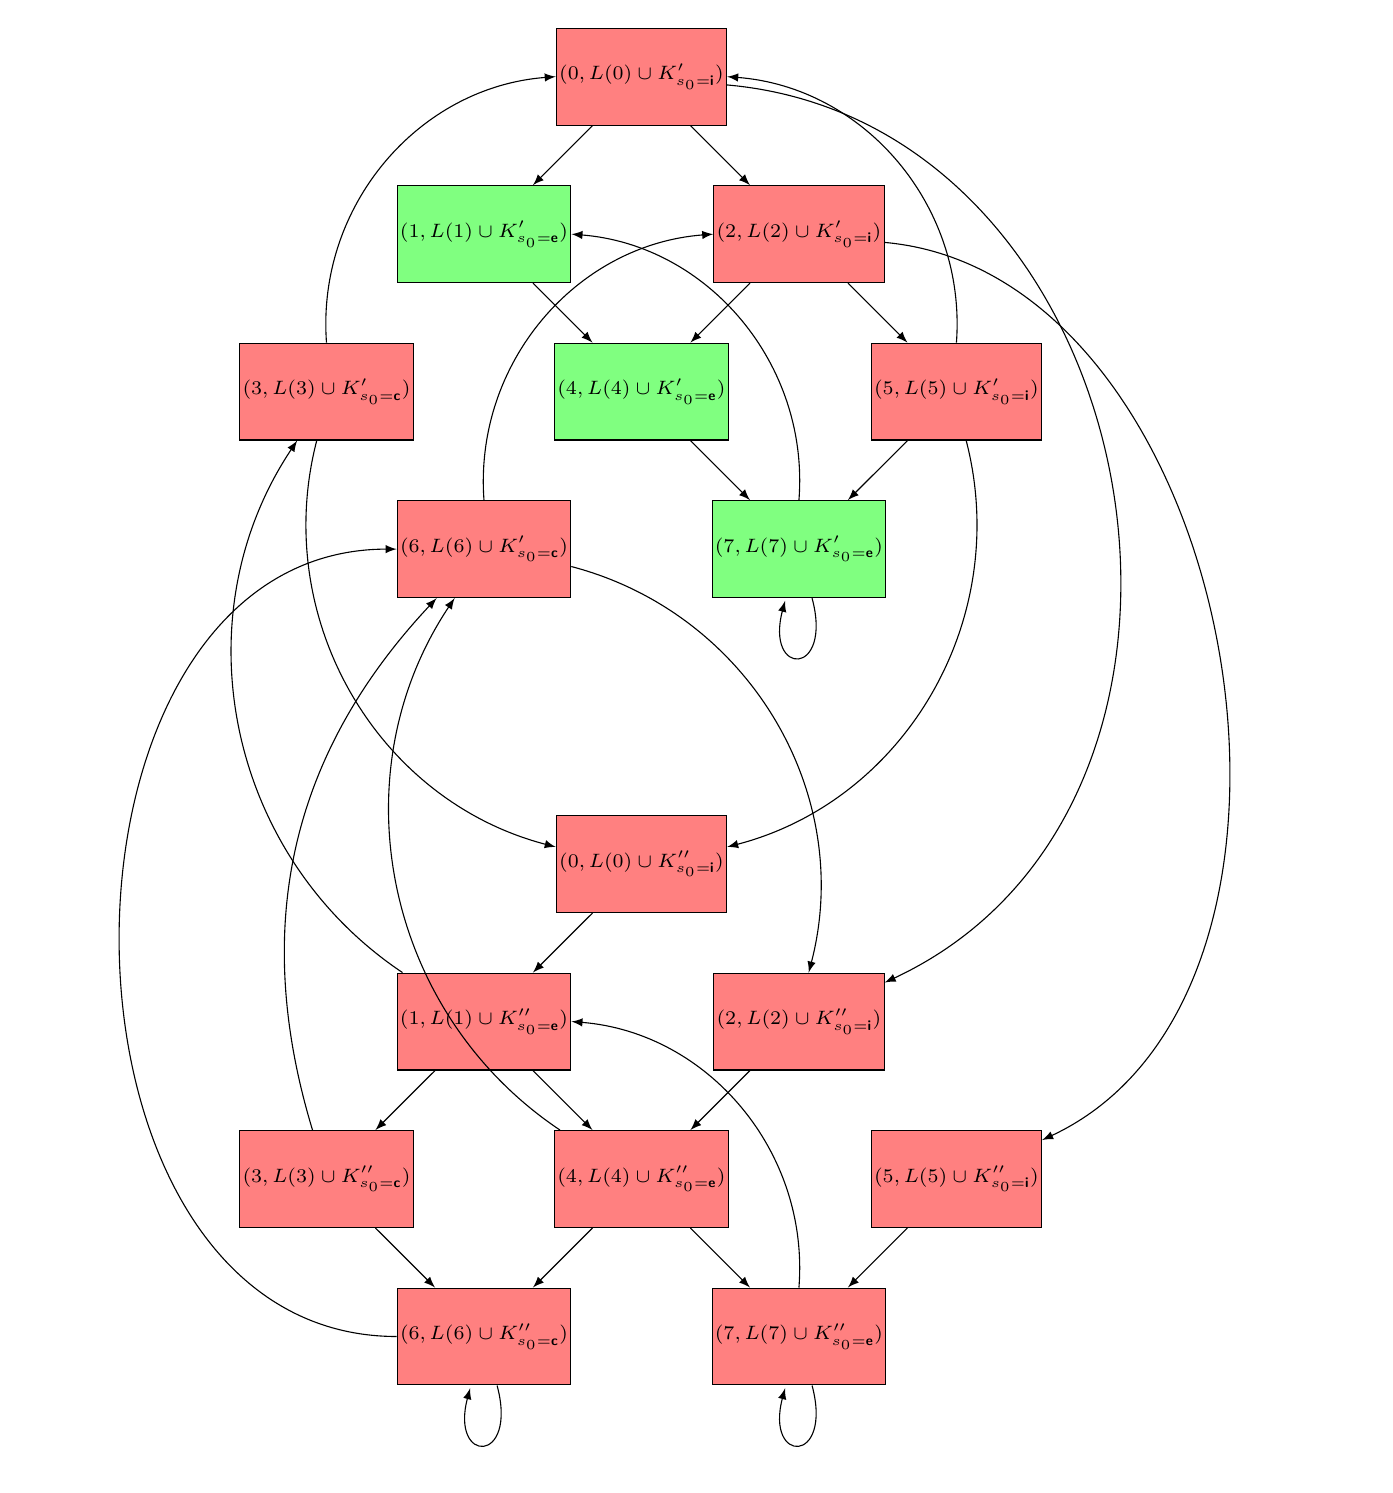
\begin{tikzpicture}[
  ->,>=latex, auto, scale=2,  every node/.style={
    rectangle, inner sep=1pt, draw, font=\scriptsize,
    align=center, minimum width=60pt, minimum height=35pt,
    SCC1/.style={fill=red!50},
    SCC2/.style={fill=green!50}
  }
]
  \node [SCC1] (S0_K') at (2, 3)
        {$(0, L(0) \cup K_{s_0=\textbf{i}}')$};
  \node [SCC2] (S1_K') at (1, 2)
        {$(1, L(1) \cup K_{s_0=\textbf{e}}')$};
  \node [SCC1] (S2_K') at (3, 2)
        {$(2, L(2) \cup K_{s_0=\textbf{i}}')$};
  \node [SCC1] (S3_K') at (0, 1)
        {$(3, L(3) \cup K_{s_0=\textbf{c}}')$};
  \node [SCC2] (S4_K') at (2, 1)
        {$(4, L(4) \cup K_{s_0=\textbf{e}}')$};
  \node [SCC1](S5_K') at (4, 1)
        {$(5, L(5) \cup K_{s_0=\textbf{i}}')$};
  \node [SCC1] (S6_K') at (1, 0)
        {$(6, L(6) \cup K_{s_0=\textbf{c}}')$};
  \node [SCC2] (S7_K') at (3, 0)
        {$(7, L(7) \cup K_{s_0=\textbf{e}}')$};

  \node [SCC1] (S0_K'') at (2, -2)
        {$(0, L(0) \cup K_{s_0=\textbf{i}}'')$};
  \node [SCC1] (S1_K'') at (1, -3)
        {$(1, L(1) \cup K_{s_0=\textbf{e}}'')$};
  \node [SCC1] (S2_K'') at (3, -3)
        {$(2, L(2) \cup K_{s_0=\textbf{i}}'')$};
  \node [SCC1] (S3_K'') at (0, -4)
        {$(3, L(3) \cup K_{s_0=\textbf{c}}'')$};
  \node [SCC1] (S4_K'') at (2, -4)
        {$(4, L(4) \cup K_{s_0=\textbf{e}}'')$};
  \node [SCC1] (S5_K'') at (4, -4)
        {$(5, L(5) \cup K_{s_0=\textbf{i}}'')$};
  \node [SCC1] (S6_K'') at (1, -5)
        {$(6, L(6) \cup K_{s_0=\textbf{c}}'')$};
  \node [SCC1] (S7_K'') at (3, -5)
        {$(7, L(7) \cup K_{s_0=\textbf{e}}'')$};

  \path
    (S0_K') edge (S1_K') edge (S2_K')
            edge [bend left =75, looseness=1.2] (S2_K'')
    (S1_K') edge (S4_K')
    (S2_K') edge (S4_K') edge (S5_K')
            edge [bend left =75] (S5_K'')
    (S3_K') edge [bend left =45] (S0_K')
            edge [bend right=45] (S0_K'')
    (S4_K') edge (S7_K')
    (S5_K') edge (S7_K') edge [bend right=45] (S0_K')
            edge [bend left =45] (S0_K'')
    (S6_K') edge [bend left =45] (S2_K')
            edge [bend left =45] (S2_K'')
    (S7_K') edge [loop below] (S7_K') edge [bend right=45] (S1_K')
    
    (S0_K'') edge (S1_K'')
    (S1_K'') edge (S3_K'') edge (S4_K'')
             edge [bend left =45] (S3_K')
    (S2_K'') edge (S4_K'')
    (S3_K'') edge (S6_K'')
             edge [bend left] (S6_K')
    (S4_K'') edge (S6_K'') edge (S7_K'')
             edge [bend left =45] (S6_K')
    (S5_K'') edge (S7_K'')
    (S6_K'') edge [loop below] (S6_K'')
             edge [bend left =90, looseness=1.2] (S6_K')
    (S7_K'') edge [loop below] (S7_K'') edge [bend right=45] (S1_K'')
    ;
\end{tikzpicture}
\end{center}

\end{document}